% Create document
\documentclass[aspectratio=1610,12pt]{beamer}
\usepackage[utf8]{inputenc}
\usepackage{csquotes}
\usepackage{tikz}
\usetikzlibrary{calc}
\usepackage{booktabs}
\usepackage[scale=2]{ccicons}
\usepackage{graphicx}
\usepackage{adjustbox}
\usepackage[flushleft]{threeparttable}
\usepackage{subcaption}
\usepackage{soul}
\usepackage[style=authoryear, backend=bibtex, dashed=false]{biblatex} % Citations

% Theme
\usetheme[progressbar=frametitle]{metropolis}
\usefonttheme{professionalfonts}

% UHH Colours
\definecolor{UHHred}{RGB}{226,0,26}
\definecolor{UHHblue}{RGB}{2,113,187}
\definecolor{UHHgrey}{RGB}{59,81,91}
\definecolor{UHHblack}{RGB}{0,0,0}
\setbeamercolor{normal text}{bg=white,fg=UHHgrey}
\setbeamercolor{alerted text}{bg=white,fg=UHHblue}
\setbeamercolor{example text}{bg=white,fg=UHHblue}

\setbeamerfont{alerted text}{family=\sffamily, series=\bfseries\boldmath}

% Footer
\setbeamertemplate{footline}{
		\hbox{%
		 \begin{beamercolorbox}[wd=0.8\paperwidth,ht=2.5ex,dp=1ex,left]{page number in head/foot}%
		\ifnum\value{section}=0{}
		\else
		{\hspace{7pt}\insertshortauthor \quad (\insertshortinstitute) \quad - \quad \insertsubtitle: \secname}
		\fi
		\end{beamercolorbox}
		\begin{beamercolorbox}[wd=.2\paperwidth,ht=2.5ex,dp=1ex,right]{page number in head/foot}
			\insertframenumber{} / \inserttotalframenumber \hspace{5pt}
		\end{beamercolorbox}
		}
		\vspace{3pt}
	}

% Arrow
\usetikzlibrary{tikzmark,decorations.pathreplacing,calc}
\newcommand\Arrow[4][0pt]{
\begin{tikzpicture}[overlay, remember picture]
\draw [UHHblue, ->,>=stealth]
   ( $ ({pic cs:#3}|-{pic cs:#2}) - (#1,5ex) $ ) --  
    node[anchor=east,xshift=5pt,text width=5cm] {#4} 
  ( $ (pic cs:#3) - (#1,0) $ );
\end{tikzpicture}}
\usetikzlibrary{arrows.meta}

% Next Year
\newcommand\NextYear{%
  \advance\year by 1 \the\year\advance\year by -1}
  
\addbibresource{IntroBib.bib}

% Title
\title{Lecture: Applied Optimization I}
\subtitle{Introduction}
\author{Dr. Tobias Vlćek}
\institute[UHH, IVLP]{UHH, Institute of Logistics, Transport and Production @Helmut Schmidt University}
\date{Wintertrimester \the\year}
%\author{Prof. Knut Haase \& Dr. Tobias Vlćek}
%\institute[UHH, IVLP]{University of Hamburg, Institute of Logistics, Transport and Production}
%\date{Winter semester \the\year /\NextYear}
%\titlegraphic{\vspace{7.2cm}\hspace{-0.30cm}\includegraphics[width=3.5cm]{uhhlogo2010.pdf}}

% Begin Presentation

\begin{document}
\maketitle
\AtBeginSection[]
{
  \begin{frame}{Table of Contents}
    \tableofcontents[currentsection]
  \end{frame}
}

\section{Introduction}

\begin{frame}[fragile]{Course Structure}
    \begin{block}{1. Lectures}
		\begin{itemize}
			\item Live lectures every Wednesday between 8.00 AM and 9.30 AM
			\item First two lectures repeat mathematical modeling and programming basics
			\item Afterward lectures discuss practical problems and their implementation
			\item Lectures are interactive $\rightarrow$ We discuss approaches during the lectures!
			\item Communication takes place via E-Mail
		\end{itemize}
    \end{block}
\end{frame}

\begin{frame}[fragile]{Course Structure}
    \begin{block}{2. Tutorials}
		\begin{itemize}
    		\item Live tutorials every Wednesday between 9.45 AM and 11.15 AM
    		\item In these tutorials we are working on assignments
    		\item Most assignments are based on applied problems of the lecture
			\item If available, please bring a laptop with Windows, macOS, or Linux!
			\item You can form groups of up to 3 students to solve assignments together
			\item Groups can submit their solution to earn bonus points for the exam
			\item Max. 0.5 point per tutorial, points only count if the mark is at least 4.0
        \end{itemize}
    \end{block}
\end{frame}

\begin{frame}[fragile]{Course Objective}
    \label{pic_bandura}
	\begin{columns}[onlytextwidth]
		\column{0.6\textwidth}
		\center
    		\begin{block}{Applied Optimization}
				\begin{itemize}
					\item Many real-world problems can be addressed thanks to mathematical models
					\item Our objective is to foster your interest in the topic and to enable you to recognize and solve problem structures on your own
					\item This includes problem understanding and implementation in software
					\item Great seminar and thesis preparation
	    			\end{itemize}
    		\end{block}
    	\column{0.4\textwidth}
    	\center
    		\begin{figure}
    			\includegraphics[width=0.7\textwidth]{images/ivan-bandura-N_FDXbXwQmc-unsplash.jpg}
    		\end{figure}
    \end{columns}
\end{frame}

\begin{frame}{Societies and Journals}
    \begin{block}{National and international societies}
    \vspace{0.07cm}
        \begin{tabular}{lp{1.0\textwidth}}
          GOR     &   Society for Operations Research in Germany\\
          INFORMS &   Institute for Operations Research and the Management Sciences \\
          IFORS   &   International Federation of OR-Societies
        \end{tabular}
    \end{block}
    
    \begin{block}{National and international journals}
        \begin{itemize}
            \item European Journal of OR
            \item Journal of the Operational Research Society
            \item Journal on Applied Analytics (before Interfaces)
            \item Management Science
            \item Operations Research
            \item OR Spectrum
        \end{itemize}
    \end{block}
\end{frame}

\section{Applications}

\begin{frame}[fragile]{Case: Brewery Production Planning}
    \center\includegraphics[width=0.7\textwidth]{images/FS.jpg}
    \begin{itemize}
         \item Lot size planning and resource utilization analysis
         \item \fullcite{mickein2022decision}
    \end{itemize}
\end{frame}

%\begin{frame}[fragile]{Case: Sales Force Deployment (Germany)}
%	\begin{columns}[onlytextwidth]
%		\column{0.5\textwidth}
%		\center
%        \footnotesize
%			\begin{itemize}
%				\item Determining  sales territory alignment, sales force sizing, sales resource allocation, and sales force location for a medical company
%                \item \fullcite{grothe_sales_2023}
%	    		\end{itemize}
%    	\column{0.5\textwidth}
%    	\center
%    		\begin{figure}
%    			\includegraphics[width=0.9\textwidth]{images/district_annot.pdf}
%    		\end{figure}
%    \end{columns}
%\end{frame}

\begin{frame}[fragile]{Case: Police Service District Planning (Germany and Belgium)}
	\begin{columns}[onlytextwidth]
		\column{0.5\textwidth}
		\center
			\begin{itemize}
				\item Improving locations and district layouts to lower the response time of emergency services
				\item \fullcite{vlcek_police_2023}
	    		\end{itemize}
    	\column{0.5\textwidth}
    	\center
    		\begin{figure}
    			\includegraphics[width=0.9\textwidth]{images/G3_C3.pdf}
    		\end{figure}
    \end{columns}
\end{frame}

\begin{frame}[fragile]{Case: Venue seating under COVID-19 distancing rules (Germany)}
  \begin{center}
      \includegraphics[width=0.40\textwidth]{images/stadium_empty.png}
      \quad
      \includegraphics[width=0.40\textwidth]{images/stadium_covid.png}
  \end{center}
    \begin{itemize}
         \item Maximizing ticket sales under COVID-19 distancing rules for a German football club
         \item Usama Dkaidik and Matthes Koch; Current research with a likely paper submission in 2024
    \end{itemize}
\end{frame}

\begin{frame}[fragile]{Case: Metro Inflow Management (Qatar)}
	\begin{columns}[onlytextwidth]
		\column{0.5\textwidth}
		\center
			\begin{itemize}
				\item Scheduling the inflow into metro stations during the world cup in Doha 2022 to prevent crowd disasters at central stations
				\item \fullcite{vlcek_controlling_2023}
            \end{itemize}
   	\column{0.5\textwidth}
    	\center
    		\begin{figure}
    	    \includegraphics[width=0.9\textwidth]{images/metro_example.png}
    		\end{figure}
    \end{columns}
\end{frame}

\begin{frame}[fragile]{Case: Split-Order Minimization in E-Commerce (Germany)}
	\begin{columns}[onlytextwidth]
		\column{0.5\textwidth}
		\center
			\begin{itemize}
				\item Lowering split-orders of e-commerce retailers through improved product-warehouse allocations
				\item \fullcite{vlcek_optimizing_2023}
	    		\end{itemize}
    	\column{0.5\textwidth}
    	\center
    		\begin{figure}
    			\includegraphics[width=0.75\textwidth]{images/optimierung_zuordnung.pdf}
    		\end{figure}
    \end{columns}
\end{frame}

\begin{frame}[fragile]{Case: Crowd Management (Mecca)}
  \begin{center}
      \includegraphics[width=0.4\textwidth]{images/HajjProjekt2.jpg}
      \includegraphics[width=0.4\textwidth]{images/HajjProjekt.jpg}
  \end{center}
    \begin{itemize}
         \item Scheduling for the Islamic pilgrimage to Mecca
         \item \fullcite{haase2016improving}
    \end{itemize}
\end{frame}

\section{Lecture Preview}

\begin{frame}[fragile]{Lecture Topics this semester}
    	\begin{enumerate}
    		\item Introduction
            \item Julia and Mathematical Modeling in JuMP
            \item Capacitated Lot Sizing Problem
			\item Vehicle Routing for Central Libraries
			\item Improving District Layouts of Police Departments
 			\item Sales Force Deployment for Medical Companies
			\item Lowering split-orders for e-commerce retailers
			\item Safety planning for the Islamic Pilgrimage to Mecca
			\item Allocating International Student to Universities
			\item Maximizing Venue Sales under COVID-19 Restrictions
            \item Controlling Passenger Flows into Metro Systems
            \item Recap Session
    	\end{enumerate}
\end{frame}

\section{Programming Language}

\begin{frame}{Julia Programming Language}
\label{pic_julia}
	\center In this lecture we are going to work in the Julia Programming Language.
	\center \begin{figure}
		 \includegraphics[width=0.5\textwidth]{images/julia-programming-language.png}
	\end{figure}
	Here are the main reasons we will use it:
\end{frame}

\begin{frame}{Julia Programming Language}
	\begin{itemize}
   		\item \textbf{Speed:} Julia was designed to be as general as Python, as statistics-friendly as R, but as fast as C++. This focus on speed allows for fast data workflows, particularly in scientific computing.
	\end{itemize}
\end{frame}

\begin{frame}{Julia Programming Language}
	\begin{itemize}
        \item \textbf{Syntax:} Despite its high-performance, Julia has a dynamically-typed syntax that is more similar to R, Matlab and Python, making it accessible and easy to learn compared to more complex programming languages.
	\end{itemize}
\end{frame}

\begin{frame}{Julia Programming Language}
	\begin{itemize}
           \item \textbf{JuMP:} Julia's seamless integration with JuMP simplifies the process of solving complex optimization problems. It provides a high-level, user-friendly interface for modeling and solving linear and nonlinear optimization problems, making it a valuable tool for operations research, data science, and engineering applications.        
	\end{itemize}
\end{frame}

\section{Algebraic Modelling}

\begin{frame}[standout]
   Do you have experience with algebraic modeling?
\end{frame}

\begin{frame}[standout]
   What is an algebraic model?
\end{frame}

\begin{frame}{Algebraic Modeling}
\begin{block}{How to learn algebraic modeling?}
    \begin{itemize}
    	\item Practice, practice, and practice!
    	\item Understand standard models and apply their approach to other problems
    	\item Develop an understanding that the constraints of the algebraic model describe the admissible solution space
    	\item Use an available standard algorithm to determine an (optimal) solution
    \end{itemize}
\end{block}
\end{frame}

\begin{frame}{Algebraic Modeling}
    \begin{block}{Central Questions}
        \begin{itemize}
    	    \item What is to be decided?
    	    \item What is relevant to the decision?
    	    \item What information is given and relevant?
    	    \item What parameters (data) are needed?
    	    \item Which variables and of which type are needed?
        \end{itemize}
    \end{block}
    \begin{block}{Model Components}
    \begin{enumerate}
    	\item Objective function
    	\item Constraints
    	\item Variables
    \end{enumerate}
	\end{block}
\end{frame}

\begin{frame}{Linear Optimization Model}
	\begin{columns}[onlytextwidth]
		\column{0.5\textwidth}
		\begin{block}{Basic Model Formulation}
			\begin{align}
   				&\text{maximize} \quad F = \sum_{j\in \mathcal{J}} c_j \times X_j
   			\end{align}
   			\quad subject to
   			\begin{align}
  				&\sum_{j\in \mathcal{J}} a_{i,j} \times X_j  \le b_i && \forall i \in \mathcal{I} \\
   				&X_j \ge 0 &&  \forall  j \in \mathcal{J} 
			\end{align}
			\vspace{0.1cm}
		\end{block}
		\column{0.4\textwidth}
				\begin{align*}
   			 		F 	&: \text{Objective function variable,}\\
   			 		X_{j}	&: \text{decision variables,}\\
   			 		\mathcal{I} &: \text{set of $i \in \mathcal{I}$,}\\
   			 		\mathcal{J} &: \text{set of $j \in \mathcal{J}$,}\\
   			 		c_{j}	&: \text{objective function coefficients,}\\
    				a_{i,j}	&: \text{parameters,}\\
    				b_{i}	&: \text{parameters}\\
				\end{align*}
	\end{columns}
\end{frame}

\begin{frame}{Graphs}
We can model and illustrate many problems with graphs (networks).
\begin{block}{Undirected Graph}
\vspace{0.15cm}
System $(N,E)$ with non-empty node set $N = \{1,...,n \}$ and
an \textbf{edge} set $E = \left\{e_1,e_2,...,e_m \right\}$.
\end{block}
\begin{itemize}
	\item The graph $G=(N,E)$ consists of 2 sets $N$ and $E$
	\item The edge set consists of 2-element subsets of the node set
	\item $e_k = \{i_k,j_k \}, k=1,...m$ with $i_k,j_k \in N$
	\item Designation of edge elements in models: $e \in E$ or $\{i,j\}\in E$.
	\item Nodes $i$ and $j$ in $e=\{i,j\}$ are called endpoints of the edge
\end{itemize}
\end{frame}

\begin{frame}{Graphs}
\begin{block}{Directed Graph}
\vspace{0.15cm}
System $(N,A)$ with non-empty node set $N = \{1,...,n \}$ and
an \textbf{arc} set $A = \left\{a_1,a_2,...,a_m \right\}$ 
\end{block}
\begin{itemize}
    \item The graph $G=(N,A)$ consists of 2 sets $N$ and $A$
	\item Edges have an orientation (start and end nodes)
	\item The edge $a=(i,j)$ is different from $a'=(j,i)$
	\item Very common in logistics
	\item Directed edge: also `arrow' or `arc' (hence the set is called $A$)
\end{itemize}
\end{frame}

\section{First Applied Case}

\begin{frame}{Solar Panel Transport}
A company is producing solar panels in Dresden and Laupheim and has to transport them to new solar farms near Hamburg, Munich, and Berlin. The quantities offered and demanded (truckloads) and the transport costs per truckload in Euro are as follows:
\begin{center}
\begin{tabular}{l|rrr|r}
\hline
Origin/Destination     & Hamburg & Munich & Berlin & Available\\
\hline
Dresden    &  5010     &  4640     &  1980   & 34\\
Laupheim   &  7120     &  1710     &  6430   & 41\\                      
\hline
Demand     &    21     &   17      &    29   &\\
\hline      
\end{tabular}
\end{center}
Example: a truckload from Dresden ($i=1$) to Munich ($j=2$) costs $c_{12}=4640$ Euro. Moreover, it is necessary to fulfil all customer demands, as the contract has already been signed.
\end{frame}

\begin{frame}[fragile]{Solar Panel Transport}
    \label{pic_kindler}
	\begin{columns}[onlytextwidth]
		\column{0.4\textwidth}
    	\center
    		\begin{figure}
    			\includegraphics[width=0.8\textwidth]{images/moritz-kindler-mRBywMReXH8-unsplash.jpg}
       		\end{figure}
		\column{0.6\textwidth}
    		\begin{block}{What could be the objective?}
            	\pause
            	Minimizing the transport costs over all truckloads while meeting the demand based on the available solar panels adhering to the available panels.
    		\end{block}
    \end{columns}
\end{frame}

\begin{frame}{Graphical Illustration}
\begin{center}
Graphically the problem can be illustrated as follows:
\boxed{
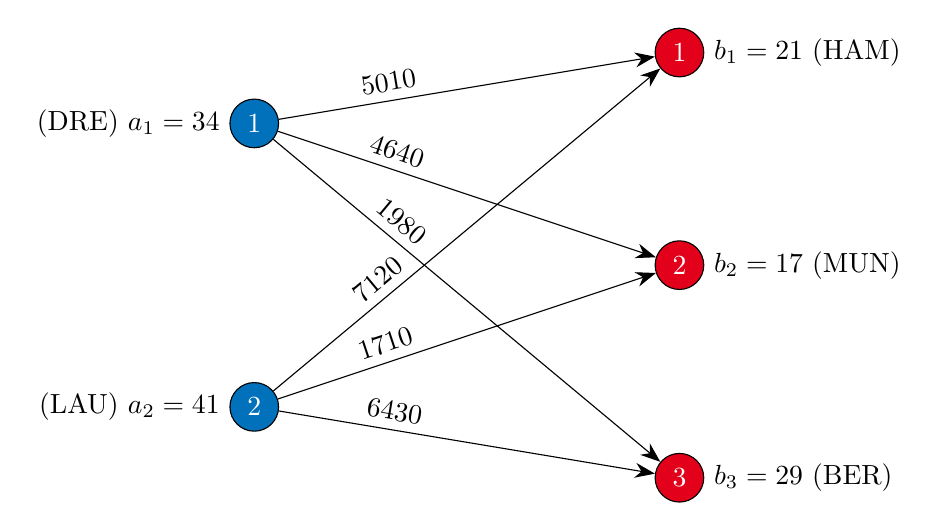
\begin{tikzpicture}[Pfeil/.style={arrows = -{Stealth[scale=1.5]}}, scale=0.9]
\coordinate (a) at (0,0);
\node[label=left:{(DRE) $a_1=34$}] (a1) at (a) [draw, circle, fill=UHHblue, text= white] {1};
\node[label=left:{(LAU) $a_2=41$}] (a2) at ($(a) - (0, 4)$) [draw, circle, fill=UHHblue, text = white] {2};
\coordinate (a) at ($(a) + (6,1)$);
\node[label=right:{$b_1=21$ (HAM)}] (b1) at (a) [draw, circle, fill=UHHred, text = white] {1};
\node[label=right:{$b_2=17$ (MUN)}] (b2) at ($(b1) - (0,3)$) [draw, circle, fill=UHHred, text = white] {2};
\node[label=right:{$b_3=29$ (BER)}] (b3) at ($(b2) - (0,3)$) [draw, circle, fill=UHHred, text = white] {3};
\draw[Pfeil] (a1) to node[sloped, above, pos=0.3]{5010} (b1);
\draw[Pfeil] (a1) to node[sloped, above, pos=0.3]{4640} (b2);
\draw[Pfeil] (a1) to node[sloped, above, pos=0.3]{1980} (b3);
\draw[Pfeil] (a2) to node[sloped, above, pos=0.3]{7120} (b1);
\draw[Pfeil] (a2) to node[sloped, above, pos=0.3]{1710} (b2);
\draw[Pfeil] (a2) to node[sloped, above, pos=0.3]{6430} (b3);
\end{tikzpicture}}
\end{center}
\end{frame}

\begin{frame}[fragile]{Available data}
\begin{block}{Sets}
\vspace{0.1cm}
	\begin{tabular}{ll}
		$\mathcal{I}$  	& set of production sites, indexed by $i$ with $i \in \{1,\ldots,|\mathcal{I}|\}$ and\\
    	$\mathcal{J}$ 	& set of customers, indexed $j$ with $j \in \{1, \ldots, |\mathcal{J}|\}$.\\
	\end{tabular}
\end{block}
\begin{block}{Parameters}
\vspace{0.1cm}
	\begin{tabular}{ll}
		$c_{i,j}$  & costs per truck load for transport from $i$ to $j$,\\
    	$a_i$ 	  & Available truck loads at $i$ and\\
    	$b_j$ 	  & Demand of customer at $j$.\\
	\end{tabular}
\end{block}
\end{frame}

\begin{frame}[fragile]{Decision variable/s}
		\begin{block}{We have the following sets:}
			\begin{itemize}
				\item All the production sites, $i \in \mathcal{I}$
				\item All customers, $j \in \mathcal{J}$
			\end{itemize}
		\end{block}
		\begin{block}{Objective}
        \vspace{0.1cm}
    	     Minimizing the transport costs over all truckloads while meeting the demand based on the available solar panels adhering to the available panels. 
    	\end{block}
    	\vspace{0.1cm}
		\begin{block}{What could be our decision variable/s?}
		\pause
			\begin{tabular}{ll}
	            $X_{i,j}$ & the number of trucks that deliver panels from site $i$ to customer $j$
			\end{tabular}
		\end{block}
\end{frame}



\begin{frame}[fragile]{Objective Function}
	\begin{columns}
		\column{0.4\textwidth}
			\boxed{
			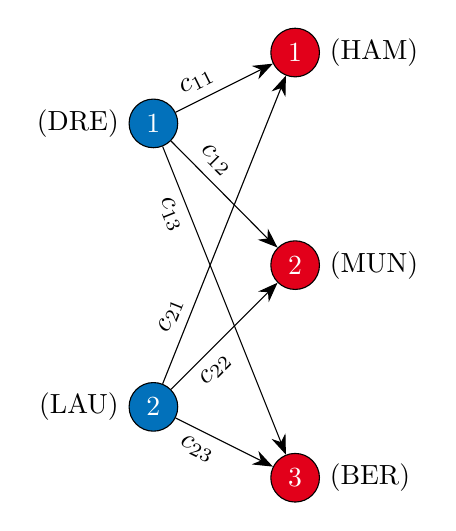
\begin{tikzpicture}[Pfeil/.style={arrows = -{Stealth[scale=1.5]}}, scale=0.9]
				\coordinate (a) at (0,0);
				\node[label=left:{(DRE)}] (a1) at (a) [draw, circle, fill=UHHblue, text= white] {1};
				\node[label=left:{(LAU)}] (a2) at ($(a) - (0, 4)$) [draw, circle, fill=UHHblue, text = white] {2};
				\coordinate (a) at ($(a) + (2,1)$);
				\node[label=right:{(HAM)}] (b1) at (a) [draw, circle, fill=UHHred, text = white] {1};
				\node[label=right:{(MUN)}] (b2) at ($(b1) - (0,3)$) [draw, circle, fill=UHHred, text = white] {2};
				\node[label=right:{(BER)}] (b3) at ($(b2) - (0,3)$) [draw, circle, fill=UHHred, text = white] {3};
				\draw[Pfeil] (a1) to node[sloped, above, pos=0.3]{$c_{11}$} (b1);
				\draw[Pfeil] (a1) to node[sloped, above, pos=0.3]{$c_{12}$} (b2);
				\draw[Pfeil] (a1) to node[sloped, below, pos=0.2]{$c_{13}$} (b3);
				\draw[Pfeil] (a2) to node[sloped, above, pos=0.2]{$c_{21}$} (b1);
				\draw[Pfeil] (a2) to node[sloped, below, pos=0.3]{$c_{22}$} (b2);
				\draw[Pfeil] (a2) to node[sloped, below, pos=0.3]{$c_{23}$} (b3);
			\end{tikzpicture}}
		\column{0.6\textwidth}
    		\begin{block}{Objective Function Transport Problem}
    				\vspace{0.1cm}
	 				Minimizing the transport costs of truckloads while meeting the demand based on the available products.\\
    				\pause
    				\vspace{0.3cm}
					\begin{tabular}{ll}
						$X_{i,j}$ & number of trucks from $i$ to $j$ and \\
	    				$c_{i,j}$ & costs for transport from $i$ to $j$.\\
					\end{tabular}\\
					\pause
					\vspace{0.4cm}
					\textbf{What could be the objective function?}
					\pause
				 	\begin{align*}
					\text{Minimize} \sum_{i \in \mathcal{I}} \sum_{j \in \mathcal{J}} c_{i,j} \times X_{i,j}
					\end{align*}
    		\end{block}
    \end{columns}
\end{frame}

\begin{frame}[fragile]{Constraints}
	\begin{columns}[onlytextwidth]
		\column{0.4\textwidth}
			\boxed{
			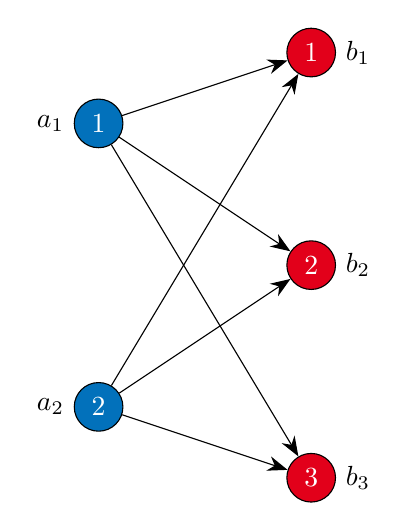
\begin{tikzpicture}[Pfeil/.style={arrows = -{Stealth[scale=1.5]}}, scale=0.9]
				\coordinate (a) at (0,0);
				\node[label=left:{$a_1$}] (a1) at (a) [draw, circle, fill=UHHblue, text= white] {1};
				\node[label=left:{$a_2$}] (a2) at ($(a) - (0, 4)$) [draw, circle, fill=UHHblue, text = white] {2};
				\coordinate (a) at ($(a) + (3,1)$);
				\node[label=right:{$b_1$}] (b1) at (a) [draw, circle, fill=UHHred, text = white] {1};
				\node[label=right:{$b_2$}] (b2) at ($(b1) - (0,3)$) [draw, circle, fill=UHHred, text = white] {2};
				\node[label=right:{$b_3$}] (b3) at ($(b2) - (0,3)$) [draw, circle, fill=UHHred, text = white] {3};
				\draw[Pfeil] (a1) to node[sloped, above, pos=0.3]{} (b1);
				\draw[Pfeil] (a1) to node[sloped, above, pos=0.3]{} (b2);
				\draw[Pfeil] (a1) to node[sloped, below, pos=0.2]{} (b3);
				\draw[Pfeil] (a2) to node[sloped, above, pos=0.2]{} (b1);
				\draw[Pfeil] (a2) to node[sloped, below, pos=0.3]{} (b2);
				\draw[Pfeil] (a2) to node[sloped, below, pos=0.3]{} (b3);
			\end{tikzpicture}}
		\column{0.6\textwidth}
    		\begin{block}{What kind of constraints do we need?}
    				\pause
    				\begin{itemize}
    					\item Ensure that the number of panels transported from a location does not exceed the available panels
    					\item We have to ensure that the demand of each customer is covered
    				\end{itemize}
    		\end{block}
    \end{columns}
\end{frame}

\begin{frame}[fragile]{Constraints}
	\begin{columns}[onlytextwidth]
		\column{0.4\textwidth}
			\boxed{
			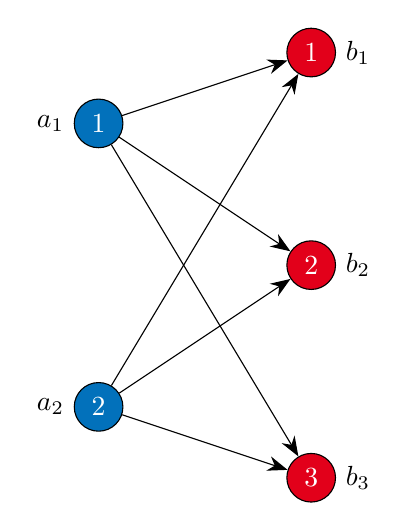
\begin{tikzpicture}[Pfeil/.style={arrows = -{Stealth[scale=1.5]}}, scale=0.9]
				\coordinate (a) at (0,0);
				\node[label=left:{$a_1$}] (a1) at (a) [draw, circle, fill=UHHblue, text= white] {1};
				\node[label=left:{$a_2$}] (a2) at ($(a) - (0, 4)$) [draw, circle, fill=UHHblue, text = white] {2};
				\coordinate (a) at ($(a) + (3,1)$);
				\node[label=right:{$b_1$}] (b1) at (a) [draw, circle, fill=UHHred, text = white] {1};
				\node[label=right:{$b_2$}] (b2) at ($(b1) - (0,3)$) [draw, circle, fill=UHHred, text = white] {2};
				\node[label=right:{$b_3$}] (b3) at ($(b2) - (0,3)$) [draw, circle, fill=UHHred, text = white] {3};
				\draw[Pfeil] (a1) to node[sloped, above, pos=0.3]{} (b1);
				\draw[Pfeil] (a1) to node[sloped, above, pos=0.3]{} (b2);
				\draw[Pfeil] (a1) to node[sloped, below, pos=0.2]{} (b3);
				\draw[Pfeil] (a2) to node[sloped, above, pos=0.2]{} (b1);
				\draw[Pfeil] (a2) to node[sloped, below, pos=0.3]{} (b2);
				\draw[Pfeil] (a2) to node[sloped, below, pos=0.3]{} (b3);
			\end{tikzpicture}}
		\column{0.6\textwidth}
    		\begin{block}{Number of panels transported from a site does not exceed the available panels}
    				\vspace{0.2cm}
    				\begin{tabular}{ll}
						$X_{i,j}$ & number of trucks from $i$ to $j$ and \\
	    				$a_{i}$ & available panels at site $i$.\\
					\end{tabular}\\
					\vspace{0.4cm}
					\pause
					\textbf{How does the constraint look like?}
					\vspace{0.2cm}
    				\pause
				 	\begin{align*}
    					&\sum_{j \in \mathcal{J}} X_{i,j} \leq {a_i} && i \in \mathcal{I}
   					\end{align*}
    		\end{block}
    \end{columns}
\end{frame}

\begin{frame}[fragile]{Constraints}
	\begin{columns}[onlytextwidth]
		\column{0.4\textwidth}
			\boxed{
			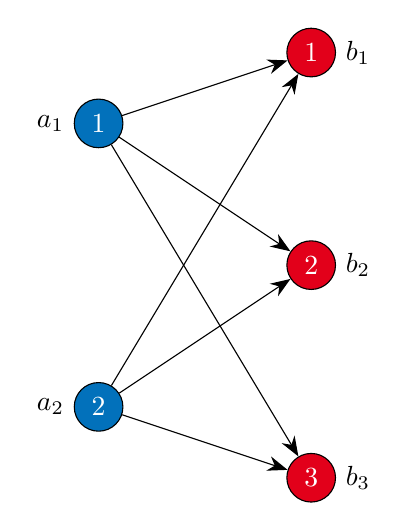
\begin{tikzpicture}[Pfeil/.style={arrows = -{Stealth[scale=1.5]}}, scale=0.9]
				\coordinate (a) at (0,0);
				\node[label=left:{$a_1$}] (a1) at (a) [draw, circle, fill=UHHblue, text= white] {1};
				\node[label=left:{$a_2$}] (a2) at ($(a) - (0, 4)$) [draw, circle, fill=UHHblue, text = white] {2};
				\coordinate (a) at ($(a) + (3,1)$);
				\node[label=right:{$b_1$}] (b1) at (a) [draw, circle, fill=UHHred, text = white] {1};
				\node[label=right:{$b_2$}] (b2) at ($(b1) - (0,3)$) [draw, circle, fill=UHHred, text = white] {2};
				\node[label=right:{$b_3$}] (b3) at ($(b2) - (0,3)$) [draw, circle, fill=UHHred, text = white] {3};
				\draw[Pfeil] (a1) to node[sloped, above, pos=0.3]{} (b1);
				\draw[Pfeil] (a1) to node[sloped, above, pos=0.3]{} (b2);
				\draw[Pfeil] (a1) to node[sloped, below, pos=0.2]{} (b3);
				\draw[Pfeil] (a2) to node[sloped, above, pos=0.2]{} (b1);
				\draw[Pfeil] (a2) to node[sloped, below, pos=0.3]{} (b2);
				\draw[Pfeil] (a2) to node[sloped, below, pos=0.3]{} (b3);
			\end{tikzpicture}}
		\column{0.6\textwidth}
    		\begin{block}{Ensure that the demand of each customer is covered}
    				\vspace{0.2cm}
    				\begin{tabular}{ll}
						$X_{i,j}$ & number of trucks from $i$ to $j$ and \\
	    				$b_{j}$ & demand at customer $i$.\\
					\end{tabular}\\
					\vspace{0.4cm}
					\pause
					\textbf{How does the constraint look like?}
					\vspace{0.2cm}
    				\pause
				 	\begin{align*}
    					&\sum_{i \in \mathcal{I}} X_{i,j} = {b_j} && j \in \mathcal{J}
   					\end{align*}
    		\end{block}
    \end{columns}
\end{frame}

\begin{frame}{Transport Problem}
	\begin{columns}[onlytextwidth]
		\column{0.15\textwidth}
		\column{0.7\textwidth}
			\begin{align}
				\text{Minimize} \quad F = \sum_{i \in \mathcal{I}} \sum_{j \in \mathcal{J}} c_{i,j} \times X_{ij}
			\end{align}
			subject to:
			\begin{align}
    			&\sum_{j \in \mathcal{J}} X_{i,j} \leq {a_i} && i \in \mathcal{I} \label{offer} \\
    			&\sum_{i \in \mathcal{I}} X_{i,j} = {b_j} && j \in \mathcal{J} \label{demand} \\
    			& X_{i,j}       \geq {0}     && i \in \mathcal{I}, j \in \mathcal{J}
			\end{align}
            \pause
            \center Could we replace $=$ by $\geq$ in equation \eqref{demand}?
		\column{0.15\textwidth}
	\end{columns}
\end{frame}

\begin{frame}[fragile]{Solar Panel Transport with Profit Maximization}
    \label{pic_pregnolato}
	\begin{columns}[onlytextwidth]
		\column{0.4\textwidth}
    	\center
    		\begin{figure}
    			\includegraphics[width=0.8\textwidth]{images/marco-pregnolato-Zir0L0GDZYY-unsplash.jpg}
       		\end{figure}
		\column{0.6\textwidth}
    		Unfortunately, the margins on solar panels are low. After the previous contract has been fulfilled, the company produced the same number of panels as before. In addition, all three customers want to order the same number of truckloads with solar panels again. The sales volume per truckload of panels is 11,000 Euros. The complete production of a truckload of solar panels, including materials, costs 6,300 Euros.\\
    		
    		In the new contract, the company wants to maximize its profits while the demand has not necessarily have to be fulfilled. What changes?
    \end{columns}
\end{frame}

\begin{frame}[fragile]{Available data}
\begin{block}{Sets}
\vspace{0.1cm}
	\begin{tabular}{ll}
		$\mathcal{I}$  	& set of production sites, indexed by $i$ with $i \in \{1,\ldots,|\mathcal{I}|\}$ and\\
    	$\mathcal{J}$ 	& set of customers, indexed $j$ with $j \in \{1, \ldots, |\mathcal{J}|\}$.\\
	\end{tabular}
\end{block}
\begin{block}{Parameters}
\vspace{0.1cm}
	\begin{tabular}{ll}
		$c_{i,j}$  & costs per truck load for transport from $i$ to $j$,\\
    	$a_i$ 	  & Available truck loads at $i$,\\
    	$b_j$ 	  & Demand of customer at $j$,\\
    	\alert{$p$} & Sales volume per truckload of solar panels and\\
    	\alert{$c$} & Production costs per truckload of solar panels.
\end{tabular}
\end{block}
\begin{block}{Variable}
\vspace{0.1cm}
	\begin{tabular}{ll}
		$X_{i,j}$ & number of trucks from $i$ to $j$. \\
\end{tabular}
\end{block}
\end{frame}

\begin{frame}[fragile]{Transport Problem}
	\begin{columns}[onlytextwidth]
		\column{0.4\textwidth}
			\boxed{
			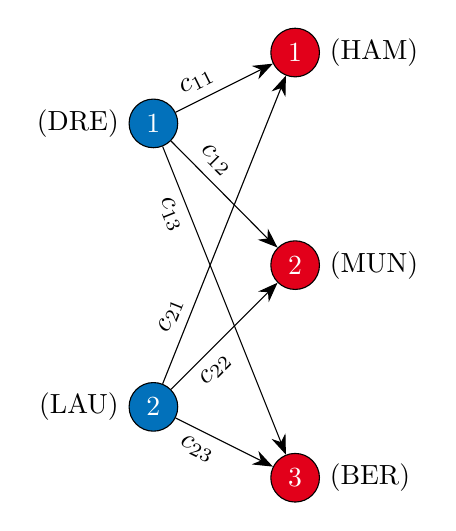
\begin{tikzpicture}[Pfeil/.style={arrows = -{Stealth[scale=1.5]}}, scale=0.9]
				\coordinate (a) at (0,0);
				\node[label=left:{(DRE)}] (a1) at (a) [draw, circle, fill=UHHblue, text= white] {1};
				\node[label=left:{(LAU)}] (a2) at ($(a) - (0, 4)$) [draw, circle, fill=UHHblue, text = white] {2};
				\coordinate (a) at ($(a) + (2,1)$);
				\node[label=right:{(HAM)}] (b1) at (a) [draw, circle, fill=UHHred, text = white] {1};
				\node[label=right:{(MUN)}] (b2) at ($(b1) - (0,3)$) [draw, circle, fill=UHHred, text = white] {2};
				\node[label=right:{(BER)}] (b3) at ($(b2) - (0,3)$) [draw, circle, fill=UHHred, text = white] {3};
				\draw[Pfeil] (a1) to node[sloped, above, pos=0.3]{$c_{11}$} (b1);
				\draw[Pfeil] (a1) to node[sloped, above, pos=0.3]{$c_{12}$} (b2);
				\draw[Pfeil] (a1) to node[sloped, below, pos=0.2]{$c_{13}$} (b3);
				\draw[Pfeil] (a2) to node[sloped, above, pos=0.2]{$c_{21}$} (b1);
				\draw[Pfeil] (a2) to node[sloped, below, pos=0.3]{$c_{22}$} (b2);
				\draw[Pfeil] (a2) to node[sloped, below, pos=0.3]{$c_{23}$} (b3);
			\end{tikzpicture}}
		\column{0.1\textwidth}
		\column{0.5\textwidth}
    		\begin{block}{What do we change in our model?}
    				\vspace{0.2cm}
    				\pause
				 	We will talk about this in more detail in the first tutorial, after we have installed the Julia Programming Language.
    		\end{block}
    \end{columns}
\end{frame}

\section{Tutorial}

\begin{frame}[fragile]{1.a. Installation of the Julia Programming Language}
\label{pic_julia}
	\begin{columns}[onlytextwidth]
		\column{0.4\textwidth}
    	\center
    		\begin{figure}
    			\includegraphics[width=0.8\textwidth]{images/julia-programming-language.png}
       		\end{figure}
		\column{0.6\textwidth}
    		To prepare for the upcoming lectures, we start by installing the Julia Programming Language and an Integrated Development Environment to work with Julia.
    \end{columns}
\end{frame}

\begin{frame}[fragile]{1.a. Installation of the Julia Programming Language}
	\begin{columns}[onlytextwidth]
		\column{0.4\textwidth}
    	\center
    		\begin{figure}
    			\includegraphics[width=0.8\textwidth]{images/julia-programming-language.png}
       		\end{figure}
		\column{0.6\textwidth}
    		If you are a windows user, head to  \url{https://julialang.org} and download and install the current stable release of Julia for your operating system. Make sure to check the box "add to path" during the installation.\\
    		\vspace{0.2cm}
    		If your are on a unix based operating system, we would recommend to pass the following code into your terminal and follow the instructions to install the Julia Up Installation Manager:\\
    		\vspace{0.1cm}
    		\$ curl -fsSL https://install.julialang.org | sh	
    \end{columns}
\end{frame}

\begin{frame}[fragile]{1.a. Installation of the IDE}
	\begin{columns}[onlytextwidth]
		\column{0.4\textwidth}
    	\center
    		\begin{figure}
    			\includegraphics[width=0.6\textwidth]{images/codium_cnl.png}
       		\end{figure}
		\column{0.6\textwidth}
    		Next, we are going to install VS Code. Alternatively, you can install VS Codium which is essentially VS Code by Microsoft but without any tracking by Microsoft in the background.\\
    		\vspace{0.2cm}
    		Head to the website \url{https://code.visualstudio.com} or \url{https://vscodium.com} and download and install the latest release for your operating system.\\
    		\vspace{0.1cm}	
    \end{columns}
\end{frame}

\begin{frame}[fragile]{1.a. Installation of the IDE}
	\begin{columns}[onlytextwidth]
		\column{0.4\textwidth}
    	\center
    		\begin{figure}
    			\includegraphics[width=0.6\textwidth]{images/codium_cnl.png}
       		\end{figure}
		\column{0.6\textwidth}
    		Great, afterwards start the IDE and check whether everything is working correctly.\\
    		\vspace{0.2cm}
    		Everything up and running? Search for the field "Extensions" on the left side bar, click it and search for "Julia". Download and install "Julia (Julia Language Support)". \\
    		\vspace{0.2cm}
    		Now, create a new file with a ".jl" ending and the content "print("Hello World!")" and save it somewhere on your computer, e.g. in a folder that you will use in the course of the lecture.
    		\vspace{0.1cm}	
    \end{columns}
\end{frame}

\begin{frame}[fragile]{1.a. Installation of the IDE}
	\begin{columns}[onlytextwidth]
		\column{0.4\textwidth}
    	\center
    		\begin{figure}
    			\includegraphics[width=0.6\textwidth]{images/codium_cnl.png}
       		\end{figure}
		\column{0.6\textwidth}
    		Run the file by clicking the "run" button in the upper right corner or by pressing "Control+Enter" or "STRG+Enter". \\
    		\vspace{0.2cm}
    		Does the terminal open with a "Hello World!"? If yes, perfect. If not, it is likely that the IDE cannot find the path to Julia. Determine the path and and save it, then try to run the file again.\\
    		\vspace{0.2cm}
    		Now we have everything set up for the next lecture. Thus, we are ready to look at the first modeling tasks in today's tutorial.
    		\vspace{0.1cm}	
    \end{columns}
\end{frame}

\begin{frame}{1.b. Solar Panel Transport}
A company is producing solar panels in Dresden and Laupheim and has to transport them to new solar farms near Hamburg, Munich, and Berlin. The quantities offered and demanded (truckloads) and the transport costs per truckload in Euro are as follows:
\begin{center}
\begin{tabular}{l|rrr|r}
\hline
Origin/Destination     & Hamburg & Munich & Berlin & Available\\
\hline
Dresden    &  5010     &  4640     &  1980   & 34\\
Laupheim   &  7120     &  1710     &  6430   & 41\\                      
\hline
Demand     &    21     &   17      &    29   &\\
\hline      
\end{tabular}
\end{center}
Example: a truckload from Dresden ($i=1$) to Munich ($j=2$) costs $c_{12}=4640$ Euro. Moreover, it is necessary to fulfill all customer demands, as the contract has already been signed.
\end{frame}

\begin{frame}{1.b. Solar Panel Transport}
	\begin{columns}[onlytextwidth]
		\column{0.15\textwidth}
		\column{0.7\textwidth}
			\begin{align}
				\text{Minimize} \quad F = \sum_{i \in \mathcal{I}} \sum_{j \in \mathcal{J}} c_{i,j} \times X_{i,j}
			\end{align}
			subject to:
			\begin{align}
    			&\sum_{j \in \mathcal{J}} X_{i,j} \leq {a_i} && i \in \mathcal{I} \\
    			&\sum_{i \in \mathcal{I}} X_{i,j} \geq {b_j} && j \in \mathcal{J} \\
    			& X_{i,j}       \geq {0}     && i \in \mathcal{I}, j \in \mathcal{J}
			\end{align}
		\column{0.15\textwidth}
	\end{columns}
\end{frame}

\begin{frame}[fragile]{1.b. Solar Panel Transport}
	\begin{columns}[onlytextwidth]
		\column{0.4\textwidth}
    	\center
    		\begin{figure}
    			\includegraphics[width=0.8\textwidth]{images/marco-pregnolato-Zir0L0GDZYY-unsplash.jpg}
       		\end{figure}
		\column{0.6\textwidth}
    		Unfortunately, the margins on solar panels are low. After the previous contract has been fulfilled, the company produced the same number of panels as before. In addition, all three customers want to order the same number of truckloads with solar panels again. The sales volume per truckload of panels is 11,000 Euros. The complete production of a truckload of solar panels, including materials, costs 6,300 Euros.\\
    		
    		In the new contract, the company wants to maximize its profits while the demand has not necessarily have to be fulfilled. What changes?
    \end{columns}
\end{frame}

\begin{frame}[fragile]{Available data}
\begin{block}{Sets}
\vspace{0.1cm}
	\begin{tabular}{ll}
		$\mathcal{I}$  	& set of production sites, indexed by $i$ with $i \in \{1,\ldots,|\mathcal{I}|\}$ and\\
    	$\mathcal{J}$ 	& set of customers, indexed $j$ with $j \in \{1, \ldots, |\mathcal{J}|\}$.\\
	\end{tabular}
\end{block}
\begin{block}{Parameters}
\vspace{0.1cm}
	\begin{tabular}{ll}
		$c_{i,j}$  & costs per truck load for transport from $i$ to $j$,\\
    	$a_i$ 	  & Available truck loads at $i$,\\
    	$b_j$ 	  & Demand of customer at $j$,\\
    	\alert{$p$} & Sales volume per truckload of solar panels and\\
    	\alert{$c$} & Production costs per truckload of solar panels.
\end{tabular}
\end{block}
\begin{block}{Variable}
\vspace{0.1cm}
	\begin{tabular}{ll}
		$X_{i,j}$ & number of trucks from $i$ to $j$. \\
\end{tabular}
\end{block}
\end{frame}

\begin{frame}[fragile]{1.b. Solar Panel Transport}
	\begin{columns}[onlytextwidth]
		\column{0.4\textwidth}
			\boxed{
			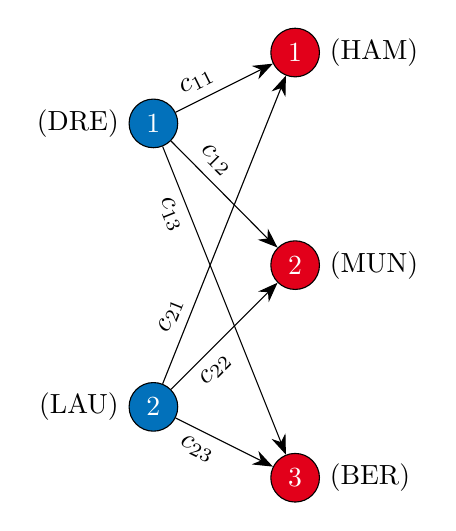
\begin{tikzpicture}[Pfeil/.style={arrows = -{Stealth[scale=1.5]}}, scale=0.9]
				\coordinate (a) at (0,0);
				\node[label=left:{(DRE)}] (a1) at (a) [draw, circle, fill=UHHblue, text= white] {1};
				\node[label=left:{(LAU)}] (a2) at ($(a) - (0, 4)$) [draw, circle, fill=UHHblue, text = white] {2};
				\coordinate (a) at ($(a) + (2,1)$);
				\node[label=right:{(HAM)}] (b1) at (a) [draw, circle, fill=UHHred, text = white] {1};
				\node[label=right:{(MUN)}] (b2) at ($(b1) - (0,3)$) [draw, circle, fill=UHHred, text = white] {2};
				\node[label=right:{(BER)}] (b3) at ($(b2) - (0,3)$) [draw, circle, fill=UHHred, text = white] {3};
				\draw[Pfeil] (a1) to node[sloped, above, pos=0.3]{$c_{11}$} (b1);
				\draw[Pfeil] (a1) to node[sloped, above, pos=0.3]{$c_{12}$} (b2);
				\draw[Pfeil] (a1) to node[sloped, below, pos=0.2]{$c_{13}$} (b3);
				\draw[Pfeil] (a2) to node[sloped, above, pos=0.2]{$c_{21}$} (b1);
				\draw[Pfeil] (a2) to node[sloped, below, pos=0.3]{$c_{22}$} (b2);
				\draw[Pfeil] (a2) to node[sloped, below, pos=0.3]{$c_{23}$} (b3);
			\end{tikzpicture}}
		\column{0.1\textwidth}
		\column{0.5\textwidth}
		\textbf{What could be the new objective of the company?} \textbf{What might we need to change in our model?}\\
		\vspace{0.2cm}
        Answer both questions. Based on the changed specification, set up an algebraic model that incorporates the novel changes.
    \end{columns}
\end{frame}

\begin{frame}[fragile]{1.c. Solar Panel Transport}
\label{pic_strauss}
	\begin{columns}[onlytextwidth]
		\column{0.4\textwidth}
    	\center
    		\begin{figure}
    			\includegraphics[width=0.8\textwidth]{images/marcel-strauss-yfhAB5ry23A-unsplash.jpg}
       		\end{figure}
		\column{0.6\textwidth}
    		Due to new manufacturing restrictions, the company will have to produce and sell the same number of solar panels from each production site in the future.
    \end{columns}
\end{frame}

\begin{frame}[fragile]{1.c. Solar Panel Transport}
	\begin{columns}[onlytextwidth]
		\column{0.4\textwidth}
			\boxed{
			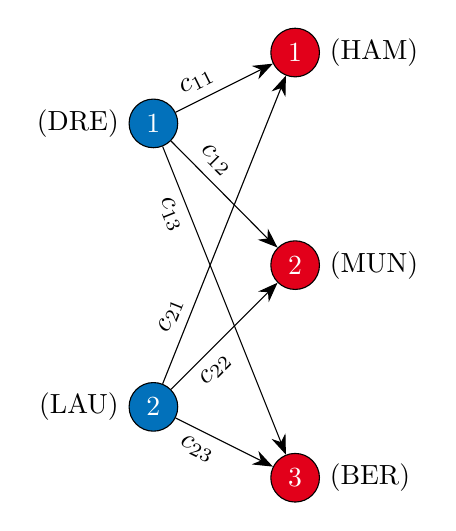
\begin{tikzpicture}[Pfeil/.style={arrows = -{Stealth[scale=1.5]}}, scale=0.9]
				\coordinate (a) at (0,0);
				\node[label=left:{(DRE)}] (a1) at (a) [draw, circle, fill=UHHblue, text= white] {1};
				\node[label=left:{(LAU)}] (a2) at ($(a) - (0, 4)$) [draw, circle, fill=UHHblue, text = white] {2};
				\coordinate (a) at ($(a) + (2,1)$);
				\node[label=right:{(HAM)}] (b1) at (a) [draw, circle, fill=UHHred, text = white] {1};
				\node[label=right:{(MUN)}] (b2) at ($(b1) - (0,3)$) [draw, circle, fill=UHHred, text = white] {2};
				\node[label=right:{(BER)}] (b3) at ($(b2) - (0,3)$) [draw, circle, fill=UHHred, text = white] {3};
				\draw[Pfeil] (a1) to node[sloped, above, pos=0.3]{$c_{11}$} (b1);
				\draw[Pfeil] (a1) to node[sloped, above, pos=0.3]{$c_{12}$} (b2);
				\draw[Pfeil] (a1) to node[sloped, below, pos=0.2]{$c_{13}$} (b3);
				\draw[Pfeil] (a2) to node[sloped, above, pos=0.2]{$c_{21}$} (b1);
				\draw[Pfeil] (a2) to node[sloped, below, pos=0.3]{$c_{22}$} (b2);
				\draw[Pfeil] (a2) to node[sloped, below, pos=0.3]{$c_{23}$} (b3);
			\end{tikzpicture}}
		\column{0.1\textwidth}
		\column{0.5\textwidth}
    		\textbf{What might we need to change in our model?}\\
    		\vspace{0.2cm}
            Based on the changed specification, set up an algebraic model that incorporates the novel changes.
    \end{columns}
\end{frame}

\section{Literature}
\begin{frame}[allowframebreaks]{Literature}
\printbibliography
\end{frame}

\begin{frame}[fragile]{Image Sources}
\footnotesize
Below a list of image sources for all images not taken by our institute:
    \begin{itemize}
        \item Slide \ref{pic_bandura}: Ivan Bandura from Unsplash
        \item Slide \ref{pic_kindler}: Moritz Kindler from Unsplash
        \item Slide \ref{pic_pregnolato}: Marco Pregnolato from Unsplash
        \item Slide \ref{pic_strauss}: Marcel Strauss from Unsplash
        \item Slide \ref{pic_julia}: JuliaLang.org
    \end{itemize}
\end{frame}
\end{document}

